
% JuliaCon proceedings template
\documentclass{juliacon}
\setcounter{page}{1}

\begin{document}

% **************GENERATED FILE, DO NOT EDIT**************

\title{ChipSort: a SIMD and cache-aware sorting module}

\author[]{Nicolau Leal Werneck}
\affil[]{TomTom NV}

\keywords{Julia, Sorting, SIMD, Parallelism, Metaprogramming}



\maketitle

\begin{abstract}

Sorting is a fundamental programming problem with many important applications, being very useful to organize data for fast retrieval. While there are well-known sorting algorithms for conventional computers, especial techniques are required to take the most out of real hardware offering features such as cache memory and instruction-level parallelism. ChipSort is a Julia module for SIMD and cache-aware sorting. It implements sorting networks and bitonic merge networks with SIMD instructions, with configurable vector sizes. It also implements Comb-sort, which lends itself easily to vectorization and achieves good performance in arrays that fit cache memory, with low penalty for random access. This also depends on a parallel in-place matrix transposition implemented in ChipSort. Large arrays are approached with a multi-way Merge-sort. The implementation of ChipSort itself is of interest from a programming languages perspective due to its use of metaprogramming, and more specifically Julia's generated functions. This enables tuning the code generation to specific tasks and hardware at runtime, a feat owed to Julia. This article presents the implemented techniques as well as experiments that demonstrate the increased speed and the hardware adaptation capability of the module.

\end{abstract}

\section{Introduction}

Sorting has enjoyed an important place within computer programming topics for a long time. Apart from having great importance for practical applications, it also attracts much attention as a theoretically interesting problem in itself~\cite{DBLP:books/lib/Knuth98a}. While sorting is a well-understood problem in general, with a few classic algorithms available, achieving optimal performance for specific problems and architectures may require a careful algorithm selection rather than just tuning parameters \cite[Part II, Introduction]{DBLP:books/daglib/0023376}.

The running time of a computer program is governed by many factors, starting with algorithmic complexity and the base clock speed of the processor. The observed performance in real computers has been increasingly depending in processor features that are not taken into account by the simplest models, though. These features include cache memory and paralellism at the processor and instruction level. Cache memory has become popular in consumer processors in the past couple of decades, allowing programs to often attain higher performance than would be possible with a simpler memory architecture, as long as memory access patterns exhibit temporal and spatial locality~\cite[Chapter 3]{Drepper07whatevery}. Writing software that can better cope with paralellism has also become necessary to exploit the full potential offered by modern and future processors~\cite{wilson2018}. 

The interest in sorting and the great relevance of cache memory and paralellism in modern computing naturally lead to research on sorting algorithms that account for these factors. Processors offering SIMD (single instruction multiple data) instructions and other forms of instruction-level parallelism started to become widely available in the early 2000s. One example is the introduction of SSE instructions in the x86 architecture~\cite[Chapter 1]{kusswurm18}. The current availability of processors with 512 bit registers underscore the need of being able to write software that exploit vector operations, not to mention GPUs. 

At the time CPUs with SIMD instructions became widely available there was already a trend to employ specialized hardware like GPUs for scientific applications~\cite{larsen2001fast,DBLP:conf/micro/ThompsonHO02}. Althoug SIMD was used mostly for multimedia applications at first~\cite{CHEN2006509,DBLP:journals/mam/SlingerlandS05}, we can cite some early alternative uses including 3D graphics~\cite{DBLP:conf/pcm/MaY02} and machine learning~\cite{DBLP:conf/europar/StreyB01}.

Apart from earlier work on parallel sorting in other architectures, the late 2000s saw the first practical demonstrations of sorting with modern consumer SIMD chips~\cite{DBLP:conf/IEEEpact/InoueMKN07,DBLP:journals/pvldb/ChhuganiNLMHCBKD08}. Most of the techniques utilized then are still employed in more recent works~\cite{DBLP:journals/pvldb/BalkesenATO13,DBLP:journals/pvldb/InoueT15}.

This article presents \verb ChipSort, a Julia module that implements SIMD and cache-aware sorting utilizing some of the techniques found in the literature. These include sorting and merging networks, the use of Comb-sort for medium sized arrays and of multi-way merging for large arrays. These techniques require not only tuning parameters such as vector and array sizes, but also generating specific code when implementing different size networks. \verb ChipSort seeks to generate efficient custom code for each task, relying on Julia metaprogramming capabilities for that.

Following Section~\ref{sec:methods} presents the techniques employed in ChipSort. Section~\ref{sec:experiments} presents experimental results assessing the performance of the module and Section~\ref{sec:conclusion} brings some concluding remarks.

\section{SIMD sorting methods}
\label{sec:methods}
%
ChipSort offers three high-level functions that can be used in applications as replacements for other sorting functions such as \verb sort  in the Julia standard library. Additional work is required from the user selecting among the three functions and also setting some numeric parameters. The functions are intended to be used with arrays of different sizes, and \verb chipsort_large  offers a good overview of all the techniques implemented in the module. Some of these techniques might also be useful in other applications instead of sorting, one clear example being the in-place matrix transpose. ChipSort does not currently support registers with separate key and payload, what might allow significant optimizations. Only the sorting of simple data types such as 32 and 64-bit integers and floating-point numbers were studied.

This section will present how \verb chipsort_large  works, detailing each step of the process. It mostly follows~\cite{DBLP:journals/pvldb/InoueT15} with a few modifications. This function achieves sorting by first splitting the input array in chunks that are sorted separately with \verb chipsort_medium!  and then merged simultaneously. This inner sort is performed in multiple steps:
\begin{enumerate}
\item sorting small blocks of data with a sorting network;
\item reordering vectors in-place according to a matrix transpose;
\item vectorized Comb-sort with a limited number of iterations;
\item regular insertion sort until the whole data is sorted.
\end{enumerate}  
The \verb chipsort_small!  function is essentially a sorting network followed by a merge procedure.

The remainder of this section will detail the multiple techniques employed in this process.

\subsection{Sorting Networks}
%
Sorting networks~\cite[Sec. 5.3.4]{DBLP:books/lib/Knuth98a} are graphs composed by comparator modules, units that take two numbers in, and output them in order: the smallest and the largest at specific outputs. Properly arranging the compatators allows the creation of a procedure that takes a vector of numbers in, and outputs them in sequence. The design of a sorting network can minimize the total number of comparisons, or also take into account that comparisons can be done in parallel, minimizing the number of steps to complete the process.

A sorting network can be represented by a Knuth graph such as Figure~\ref{fig:sorting-network}. The graph represents a network that takes an array of four values $(A_1, A_2, A_3, A_4)$ and outputs the sorted sequence $(S_1, S_2, S_3, S_4)$. Each vertical line in the graph represents a comparator.
\begin{figure}[htb]
\centerline{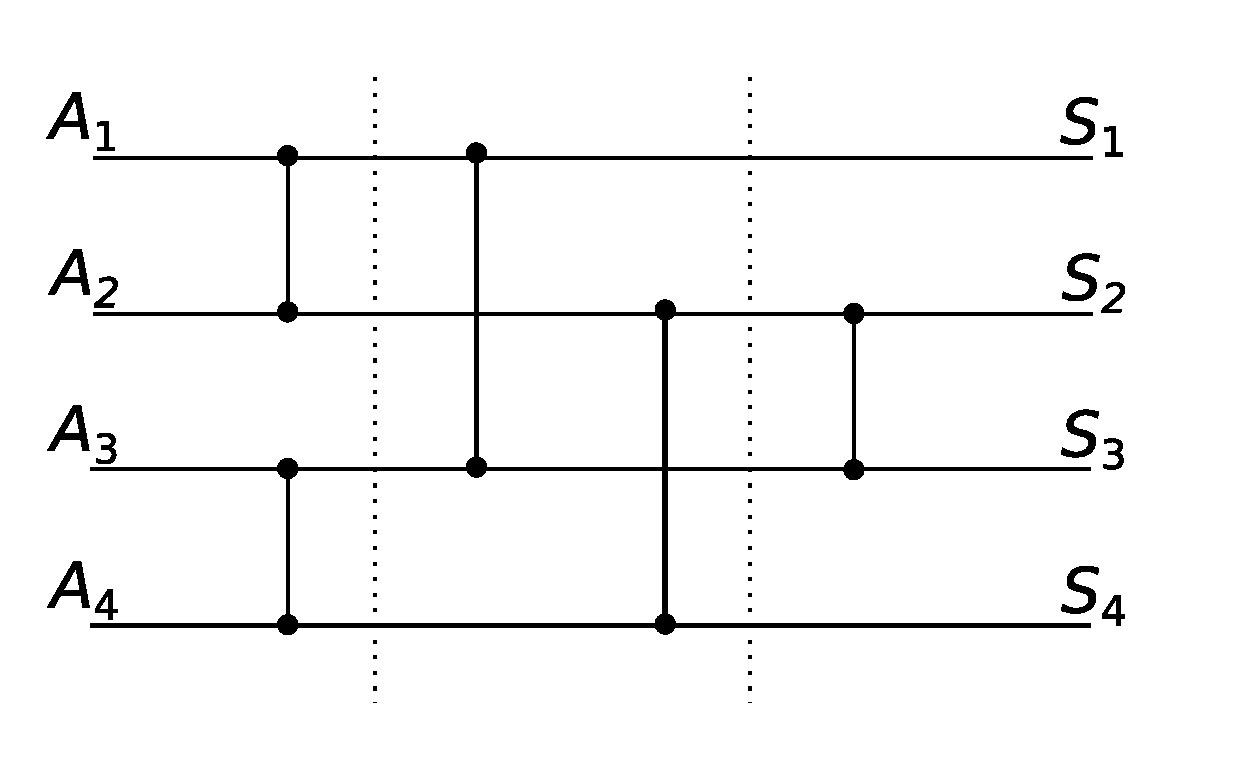
\includegraphics[width=0.9\linewidth]{fig/sorting-network-4.pdf}}
\caption{A sorting network for 4 elements. The dashed lines represent sections where operations are independent of each other.}
\label{fig:sorting-network}
\end{figure}

In ChipSort, as in the related work, parallelism is mainly exploited by carrying out the comparisons of the sorting network over vectors of size $V$ contained in SIMD registers, effectively running the network $V$ times simultaneously. Other forms of instruction-level parallelism can also be in play, though. In especial, it may also be possible to parallelize instructions such as \verb min  and \verb max , and also the loading of data into registers. This is often done implicitly by the microarchitecture, and programmers can only try to make sure their code is suitable for this by properly ordering operations and avoiding branching, for instance. Part of this work is expected to be performed by the compiler, and especially LLVM in the case of Julia.

ChipSort supports sorting networks of different sizes, currently only powers of 2, which are predefined as data structures in the file \href{https://github.com/nlw0/ChipSort.jl/blob/d2d049b7413f0073476021fa62fb748803130768/src/sorting-network-parameters.jl}{\tt sorting-network-parameters.jl}. The generated function \href{https://github.com/nlw0/ChipSort.jl/blob/d2d049b7413f0073476021fa62fb748803130768/src/sorting-networks.jl#L13}{\tt sort\_net} works by assigning each element of the sequence at each step to a variable, and calculating values from the next step according to the network specification. The comparisons are performed by the {\tt min} and {\tt max} functions, and the function is generic on the element types. Figure~\ref{fig:sort-net-listing}

\begin{figure}[htb]
\begin{lstlisting}[language = Julia]
input_0_1 = Base.getindex(input, 1)
input_0_2 = Base.getindex(input, 2)
input_0_3 = Base.getindex(input, 3)
input_0_4 = Base.getindex(input, 4)
input_1_1 = ChipSort.min(input_0_1, input_0_2)
input_1_2 = ChipSort.max(input_0_1, input_0_2)
input_1_3 = ChipSort.min(input_0_3, input_0_4)
input_1_4 = ChipSort.max(input_0_3, input_0_4)
input_2_1 = ChipSort.min(input_1_1, input_1_3)
input_2_3 = ChipSort.max(input_1_1, input_1_3)
input_2_2 = ChipSort.min(input_1_2, input_1_4)
input_2_4 = ChipSort.max(input_1_2, input_1_4)
input_3_1 = input_2_1
input_3_4 = input_2_4
input_3_2 = ChipSort.min(input_2_2, input_2_3)
input_3_3 = ChipSort.max(input_2_2, input_2_3)
return (input_3_1, input_3_2, input_3_3, input_3_4)
\end{lstlisting}
\caption{Code generated by {\tt sort\_net} to implement a 4-element sorting network.}
\label{fig:sort-net-listing}
\end{figure}

This function is a good first example of the utilization of Julia's meta-programming features in ChipSort. Multiple implementations of sorting networks are available~\cite{DBLP:journals/pvldb/ChhuganiNLMHCBKD08,sortingnetworksjl,ultrasort}, however they implement networks of different sizes straight as code. In ChipSort they are represented as data structures that guide a generated function that produces equivalent code. While this data structure currently is hard-coded, it can potentially be produced only when necessary by an implementation of an algorithm such as Bose-Nelson, what remains a future plan for the module.

The {\tt sort\_net} generated function expects elements that have defined {\tt max } and {\tt min} methods. It can be called with simple data types, {\em e.g.} {\tt sort\_net(4,2,5,3)} works. In practice ChipSort often calls this function with vectors, completely relying on SIMD.jl~\cite{erik_schnetter_2019_2592633}. This module maps a vector in Julia similar to tuples or static arrays straight to LLVM vector types, ensuring SIMD code can be produced when possible.

\subsection{SIMD}

When applied to a group of vectors, the result from the sorting network contains sorted sequences in the lanes of the vectors. To obtain sorted vectors we need to transpose these vectors.



\subsection{Bitonic Merge Networks}
%
\subsection{Vectorized Comb-sort}
%
\subsection{In-place matrix transpose}
%
\subsection{Vectorized multi-way array merging}
%

\section{Experiments}
\label{sec:experiments}
%
\section{Conclusion}
\label{sec:conclusion}
%


The \LaTeX{} document preparation system is a special version of the
\TeX; typesetting program where-in a collection of \TeX; commands
are added to \LaTeX{} to simplify typesetting. Importantly, it allows
the author to concentrate on the logical structure of the document
rather than its visual layout.\vskip 6pt
Moreover, \LaTeX{} provides a consistent and comprehensive document
preparation interface. There are simple-to-use commands for
generating a table of contents, lists of figures and/or tables, and indexes.
\LaTeX{} can automatically number list entries, equations, figures,
tables, and footnotes, as well as articles, sections, and subsections.
Using this numbering system, bibliographic citations, page
references, and cross references to any other numbered entity (e.g.
article, section, equation, figure, list entry, etc.) become quite simple
and straightforward. The use of \LaTeX{} document classes allows
a simple change of class to transform the appearance of your document.\vskip 6pt
\LaTeX{} is a powerful tool for managing long and complex documents.
In particular, partial processing enables long documents to
be produced article by article without losing sequential information.
The use of document classes allows a simple change of style
(or style option) to transform the appearance of your document.



\section{The JuliaCon Article Class}
\label{sec:documentclass}
%
The juliacon class file preserves the standard LATEX{} interface such
that any document that can be produced using the standard LATEX{}
article class can also be produced with the class file.\vskip 6pt
It is likely that the make up will change after file submission. For
this reason, we ask you to ignore details such as slightly long lines,
page stretching, or figures falling out of synchronization, as these
details can be dealt with at a later stage.\vskip 6pt
Use should be made of symbolic references (\verb \ref ) in order to
protect against late changes of order, etc.

\section{USING THE JuliaCon Article CLASS FILE}

If the file \verb juliacon.cls  is not already in the appropriate system directory
for \LaTeX{} files, either arrange for it to be put there or copy
it to your working directory. The \verb juliacon  document class is implemented
as a complete class, not a document style option. In order to
use the \verb juliacon  document class, replace \verb article  by \verb juliacon  in the
\verb \documentclass  command at the beginning of your document:
\vskip 6pt
\begin{centering}
    \verb \documentclass{article}  \end{centering}
\vskip 6pt
replace by
\vskip 6pt
 \verb \documentclass{juliacon}  \vskip 6pt
In general, the following standard document \verb style  options should
{ \itshape not} be used with the {\footnotesize \itshape article} class file:
\begin{enumerate}
\item[(1)] \verb 10pt,  \verb 11pt,  \verb 12pt   ? unavailable;
\item[(2)] \verb twoside  (no associated style file) ? \verb twoside  is the default;
\item[(3)] \verb fleqn, \verb leqno, \verb titlepage ? should not be used;
\end{enumerate}

\section{Additional Document Style Options}
\label{sec:additional_doc}
%
The following additional style option is available with the \verb juliacon  class file:
\vskip 6pt
Please place any additional command definitions at the very start of
the \LaTeX{} file, before the \verb \begin{document} . For example, user-defined
\verb \def  and \verb \newcommand   commands that define macros for
technical expressions should be placed here. Other author-defined
macros should be kept to a minimum.
\vskip 6pt
Commands that differ from the standard \LaTeX{} interface, or that
are provided in addition to the standard interface, are explained in
this guide. This guide is not a substitute for the \LaTeX{} manual itself.
Authors planning to submit their papers in \LaTeX{} are advised to use
\verb \juliacon.cls  as early as possible in the creation of their files.

%
%
%
%
\begin{table*}[t]
\tabcolsep22pt
\tbl{If necessary, the tables can be extended both columns.}{
\begin{tabular}{|l|l|c|c|}\hline
Label & \multicolumn{1}{c|}{Description}
& Number of Users &
Number of Queries\\\hline
Test 1 & Training Data &
\smash{\raise-7pt\hbox{70}} & 104\\
\cline{1-2}\cline{4-4}
Test 2 & Testing Data I & & 105\\\hline
Test 3 & Testing Data II & 30 & 119\\\hline
& Total & 100 & 328\\\hline
\end{tabular}}
\label{tab:symbols}
\begin{tabnote}
This is an example of table footnote.
\end{tabnote}
\end{table*}
% \begin{figure*}[t]
% \centerline{\includegraphics[width=11cm]{juliagraphs.png}}
% \caption{If necessary, the images can be extended both columns.}
%   \label{fig:sample_image}
% \end{figure*}

\section{Additional features}
\label{sec:additional_faci}
In addition to all the standard \LaTeX{} design elements, the \verb juliacon  class file includes the following features:
In general, once you have used the additional \verb juliacon.cls facilities
in your document, do not process it with a standard \LaTeX{} class
file.

\subsection{Titles, Author's Name, and Affiliation}
\label{subsub:title_auth}
The title of the article, author's name, and affiliation are used at the
beginning of the article (for the main title). These can be produced
using the following code:

\begin{verbatim}
\title{ This is an example of article title} }
\author{
   \large 1st Author \\[-3pt]
   \normalsize 1st author's affiliation  \\[-3pt]
    \normalsize 1st line of address \\[-3pt]
    \normalsize 2nd line of address \\[-3pt]
    \normalsize	1st author's email address \\[-3pt]
  \and
   \large 2nd Author \\[-3pt]
   \normalsize 2nd author's affiliation  \\[-3pt]
    \normalsize 1st line of address \\[-3pt]
    \normalsize 2nd line of address \\[-3pt]
    \normalsize	2nd author's email address \\[-3pt]
\and
   \large 3rd Author \\[-3pt]
   \normalsize 3rd author's affiliation  \\[-3pt]
    \normalsize 1st line of address \\[-3pt]
    \normalsize 2nd line of address \\[-3pt]
    \normalsize	3rd author's email address \\[-3pt]
}
\maketitle
\end{verbatim}

\subsection{Writing Julia code}

A special environment is already defined for Julia code,
built on top of \textit{listings} and \textit{jlcode}.

\begin{verbatim}
\begin{lstlisting}[language = Julia]
using Plots

x = -3.0:0.01:3.0
y = rand(length(x))
plot(x, y)
\end{lstlisting}
\end{verbatim}
\begin{lstlisting}[language = Julia]
using Plots

x = -3.0:0.01:3.0
y = rand(length(x))
plot(x, y)
\end{lstlisting}


\subsection{Abstracts, Key words, term etc...}
\label{subsub:abs_key_etc}

At the beginning of your article, the title should be generated
in the usual way using the \verb \maketitle  command. For genaral tem and keywords use
\verb \terms ,
\verb \keywords  commands respectively. The abstract should be enclosed
within an abstract environment, All these environment
can be produced using the following code:
\begin{verbatim}
\terms{Experimentation, Human Factors}

\keywords{Face animation, image-based modelling...}

\begin{abstract}
In this paper, we propose a new method for the
systematic determination of the model's base of
time varying delay system. This method based on
the construction of the classification data related
to the considered system. The number, the orders,
the time delay and the parameters of the local
models are generated automatically without any
knowledge about the full operating range of the
process. The parametric identification of the local
models is realized by a new recursive algorithm for
on line identification of systems with unknown time
delay. The proposed algorithm allows simultaneous
estimation of time delay and parameters of
discrete-time systems. The effectiveness of
the new method has been illustrated through
simulation.
\end{abstract}

\end{verbatim}

\section{Some guidelines}
\label{sec:some_guide}
The following notes may help you achieve the best effects with the
\verb juliacon  class file.

\subsection{Sections}
\label{subsub:sections}
\LaTeXe{}  provides four levels of section headings and they are all
defined in the \verb juliacon  class file:
\begin{itemize}
\item \verb \section   \item \verb \subsection  \item \verb \subsubsection  \item \verb \paragraph  \end{itemize}
Section headings are automatically converted to allcaps style.
\subsection{Lists}
\label{sec:lists}
%
The \verb juliacon   class file provides unnumbered lists using the
\verb unnumlist  environment for example,

\begin{unnumlist}
\item First unnumbered item which has no label and is indented from the
left margin.
\item Second unnumbered item.
\item Third unnumbered item.
\end{unnumlist}
The unnumbered list which has no label and is indented from the
left margin. was produced by:
\begin{verbatim}
\begin{unnumlist}
\item First unnumbered item...
\item Second unnumbered item...
\item Third unnumbered item...
\end{unnumlist}
\end{verbatim}

The \verb juliacon   class file also provides hyphen list using the
\verb itemize  environment for example,
\begin{itemize}
\item First unnumbered bulleted item which has no label and is indented
from the left margin.
\item Second unnumbered bulleted item.
\item Third unnumbered bulleted item which has no label and is indented
from the left margin.
\end{itemize}
was produced by:
\begin{verbatim}
\begin{itemize}
\item First item...
\item Second item...
\item Third item...
\end{itemize}
\end{verbatim}

Numbered list is also provided in acmtog class file using the
enumerate environment for example,
\begin{enumerate}
\item The attenuated and diluted stellar radiation.
\item Scattered radiation, and
\item Reradiation from other grains.
\end{enumerate}

was produced by:
\begin{verbatim}
\begin{enumerate}
\item The attenuated...
\item Scattered radiation, and...
\item Reradiation from other grains...
\end{enumerate}
\end{verbatim}
\subsection{Illustrations (or figures)}
\label{subsub:sec_Illus}
The \verb juliacon   class file will cope with most of the positioning of
your illustrations and you should not normally use the optional positional
qualifiers on the \verb figure   environment that would override
these decisions.
\vskip 6pt

%
\begin{figure}[t]
\centerline{\includegraphics[width=4cm]{juliagraphs.png}}
\caption{This is example of the image in a column.}
	\label{fig:sample_figure}
\end{figure}

The figure \ref{fig:sample_figure} is taken from the JuliaGraphs
organization \footnote{https://github.com/JuliaGraphs}.

Figure captions should be \emph{below} the figure itself, therefore the
\verb \caption  command should appear after the figure or space left for
an illustration. For example, Figure 1 is produced using the following
commands:

\begin{verbatim}
\begin{figure}
\centerline{\includegraphics[width=20pc]{Graphics.eps}}
\caption{An example of the testing process for a
binary tree. The globa null hypothesis is tested
first at level $\alpha$ (a), and the level of
individual variables is reached last (d). Note
that individual hypotheses can be tested at
level $\alpha/4$ and not $\alpha/8$ as one might
expect at first.}
\label{sample-figure_2}
\end{figure}
\end{verbatim}
Figures can be resized using first and second argument of
\verb \includegraphics   command. First argument is used for modifying
figure height and the second argument is used for modifying
figure width respectively.
\vskip 6pt
Cross-referencing of figures, tables, and numbered, displayed
equations using the \verb \label  and \verb \ref   commands is encouraged.
For example, in referencing Figure 1 above, we used
\verb Figure~\ref{sample-figure}   \subsection{Tables}
\label{subsub:sec_Tab}
The \verb juliacon   class file will cope with most of the positioning of
your tables and you should not normally use the optional positional qualifiers on the table environment which would override these
decisions. Table captions should be at the top.
\begin{verbatim}
\begin{table}
\tbl{Tuning Set and Testing Set}{
\begin{tabular}{|l|l|c|c|}\hline
Label & \multicolumn{1}{c|}{Description}
& Number of Users &
Number of Queries\\\hline
Train70 & Training Data &
\smash{\raise-7pt\hbox{70}} & 104\\
\cline{1-2}\cline{4-4}
Test70 & Testing Data I & & 105\\\hline
Test30 & Testing Data II & 30 & 119\\\hline
& Total & 100 & 328\\\hline
\end{tabular}}
\end{table}\end{verbatim}

\begin{table}
\tbl{Tuning Set and Testing Set}{
\begin{tabular}{|l|l|c|c|}\hline
Label & \multicolumn{1}{c|}{Description}
& Number of Users &
Number of Queries\\\hline
Test 1 & Training Data &
\smash{\raise-7pt\hbox{70}} & 104\\
\cline{1-2}\cline{4-4}
Test 2 & Testing Data I & & 105\\\hline
Test 3 & Testing Data II & 30 & 119\\\hline
& Total & 100 & 328\\\hline
\end{tabular}}
\end{table}
\subsection{Landscaping Pages}
\label{subsub:landscaping_pages}
If a table is too wide to fit the standard measure, it may be turned,
with its caption, to 90 degrees. Landscape tables cannot be produced
directly using the \verb juliacon   class file because \TeX{} itself cannot
turn the page, and not all device drivers provide such a facility.
The following procedure can be used to produce such pages.
\vskip 6pt
Use the package \verb rotating   in your document and change the coding
from
\begin{verbatim}
\begin{table}...\end{table}
to
\begin{sidewaystable}...\end{sidewaystable}
and for figures
\begin{figure}...\end{figure}
to
\begin{sidewaysfigure}...\end{sidewaysfigure}
\end{verbatim}

environments in your document to turn your table on the appropriate
page of your document. For instance, the following code prints
a page with the running head, a message half way down and the
table number towards the bottom.
\begin{verbatim}
\begin{sidewaystable}
\tbl{Landscape table caption to go here.}{...}
\label{landtab}
\end{sidewaystable}
\end{verbatim}

\subsection{Double Column Figure and Tables}
\label{subsub:double_fig_tab}
For generating the output of figures and tables in double column
we can use the following coding:

\begin{enumerate}
\item For Figures:
\begin{verbatim}
\begin{figure*}...\end{figure*}
\end{verbatim}
\item For landscape figures:
\begin{verbatim}
\begin{sidewaysfigure*}...\end{sidewaysfigure*}
\end{verbatim}
\item For Tables:
\begin{verbatim}
\begin{table*}...\end{table*}
\end{verbatim}
\item For landscape tables:
\begin{verbatim}
\begin{sidewaystable*}...\end{sidewaystable*}
\end{verbatim}
\end{enumerate}

\subsection{Typesetting Mathematics}
\label{subsub:type_math}
The \verb juliacon class file will set displayed mathematics with center to
the column width, provided that you use the \LaTeXe{} standard of
open and closed square brackets as delimiters.
The equation
\[
\sum_{i=1}^p \lambda_i = (S)
\]

was typeset using the acmtog class file with the commands

\begin{verbatim}
\[
\sum_{i=1}^p \lambda_i = (S)
\]
\end{verbatim}

For display equations, cross-referencing is encouraged. For example,
\begin{verbatim}
\begin{equation}
(n-1)^{-1} \sum^n_{i=1} (X_i - \overline{X})^2.
\label{eq:samplevar}
\end{equation}
Equation~(\ref{eq:samplevar}) gives the formula for
sample variance.
\end{verbatim}
The following output is generated with the above coding:
\begin{equation}
(n-1)^{-1} \sum^n_{i=1} (X_i - \overline{X})^2.
\label{eq:samplevar}
\end{equation}
Equation~(\ref{eq:samplevar}) gives the formula for
sample variance.


\subsection{Enunciations}
\label{subsub:enunciation}
The \verb juliacon   class file generates the enunciations with the help of
the following commands:
\begin{verbatim}
\begin{theorem}...\end{theorem}
\begin{strategy}...\end{strategy}
\begin{property}...\end{property}
\begin{proposition}...\end{proposition}
\begin{lemma}...\end{lemma}
\begin{example}...\end{example}
\begin{proof}...\end{proof}
\begin{definition}...\end{definition}
\begin{algorithm}...\end{algorithm}
\begin{remark}...\end{remark}
\end{verbatim}
The above-mentioned coding can also include optional arguments
such as
\begin{verbatim}
\begin{theorem}[...]. Example for theorem:
\begin{theorem}[Generalized Poincare Conjecture]
Four score and seven ... created equal.
\end{theorem}
\end{verbatim}

\begin{theorem}[Generalized Poincare Conjecture]
Four score and seven years ago our fathers brought forth,
upon this continent, a new nation, conceived in Liberty,
 and dedicated to the proposition that all men are
created equal.
\end{theorem}


\subsection{Extract}
\label{subsub:extract}
Extract environment should be coded within
\begin{verbatim}
\begin{extract}..\end{extract}
\end{verbatim}

\subsection{Balancing column at last page}
\label{subsub:Balance}
For balancing the both column length at last page use :
\begin{verbatim}
\vadjust{\vfill\pagebreak}
\end{verbatim}

%\vadjust{\vfill\pagebreak}

at appropriate place in your \TeX{} file or in bibliography file.

\section{Handling references}
\label{subsub:references}
References are most easily (and correctly) generated using the
BIBTEX, which is easily invoked via
\begin{verbatim}
\bibliographystyle{juliacon}
\bibliography{ref}
\end{verbatim}
When submitting the document source (.tex) file to external
parties, the ref.bib file should be sent with it.
\cite{bezanson2017julia}

\input{bib.tex}

\end{document}

% Inspired by the International Journal of Computer Applications template

% latexmk -bibtex -pdf paper.tex
